\chapter{Dados Coletados de 10/09/2017 a 13/11/2017}
\label{DataCollected}

\begin{figure}[H]
	\centering
	\caption{Resumo do Módulo do Aquário}
	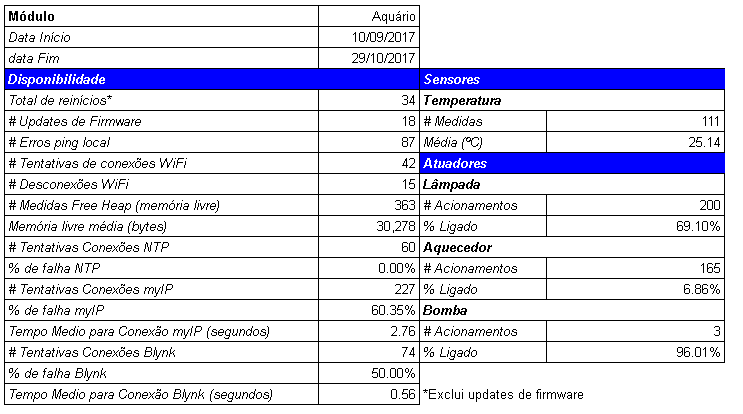
\includegraphics[width=1.0\textwidth]{resumoAqua}
	\label{fig:resumoAqua}
\end{figure}

\begin{figure}[H]
	\centering
	\caption{Disponibilidade do Módulo do Aquário -- período}
	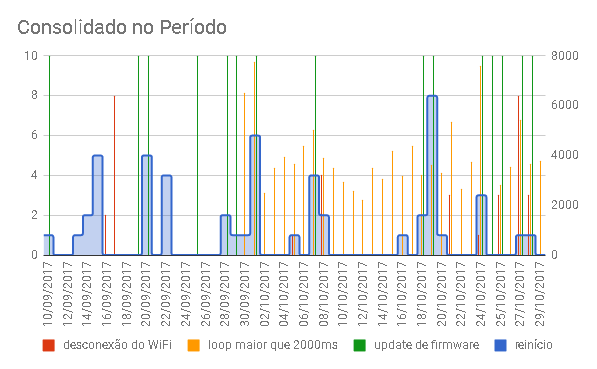
\includegraphics[width=0.8\textwidth]{AquaPeriodo}
	\label{fig:AquaPeriodo}
\end{figure}

\begin{figure}[H]
	\centering
	\caption{Disponibilidade do Módulo do Aquário -- dia}
	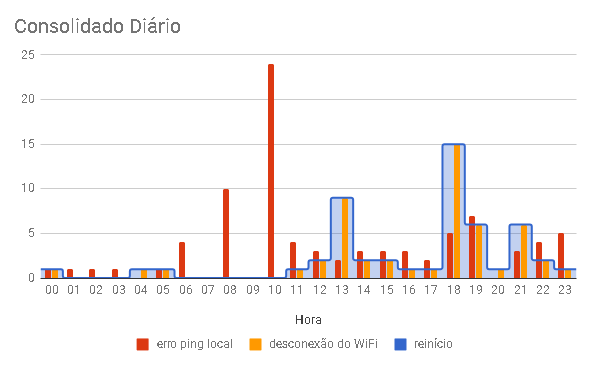
\includegraphics[width=0.8\textwidth]{AquaDiaDisp}
	\label{fig:AquaDiaDisp}
\end{figure}

\begin{figure}[H]
	\centering
	\caption{Memória livre do Módulo do Aquário}
	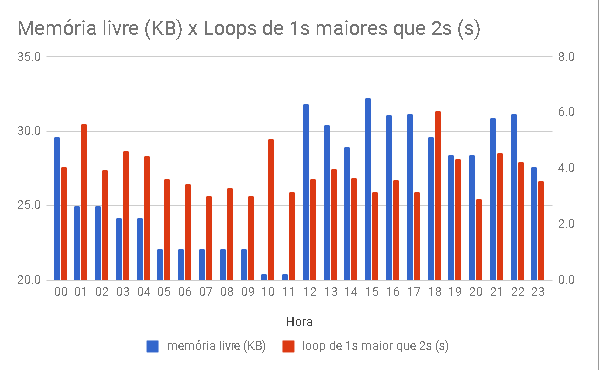
\includegraphics[width=0.8\textwidth]{MemLivreAqua}
	\label{fig:MemLivreAqua}
\end{figure}

\begin{figure}[H]
	\centering
	\caption{Resumo do Módulo do Corredor}
	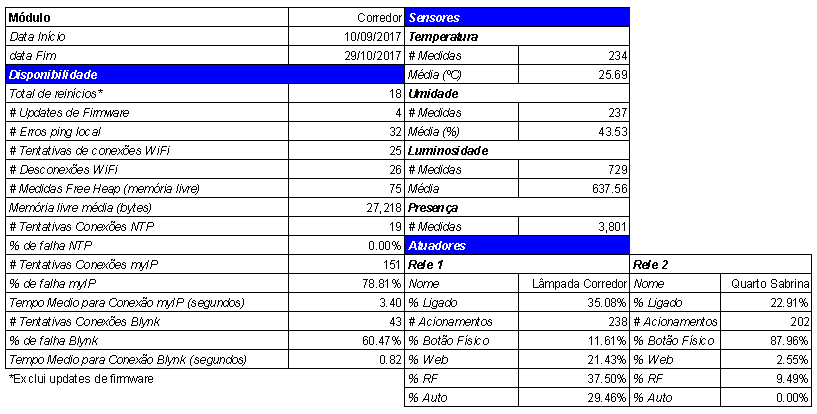
\includegraphics[width=1.0\textwidth]{resumoCorredor}
	\label{fig:resumoCorredor}
\end{figure}

\begin{figure}[H]
	\centering
	\caption{Sensores do Módulo do Corredor -- período}
	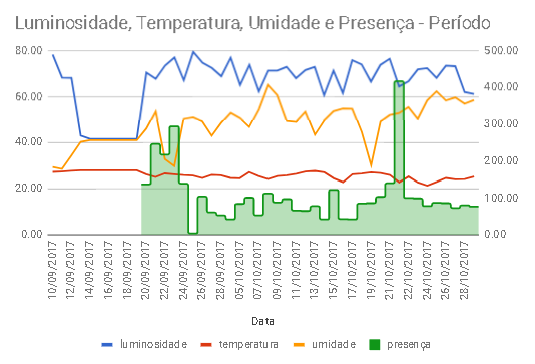
\includegraphics[width=0.8\textwidth]{sensoresperiodoCorredor}
	\label{fig:sensoresperiodoCorredor}
\end{figure}

\begin{figure}[H]
	\centering
	\caption{Uso do relê 2 -- Módulo do Corredor -- dia}
	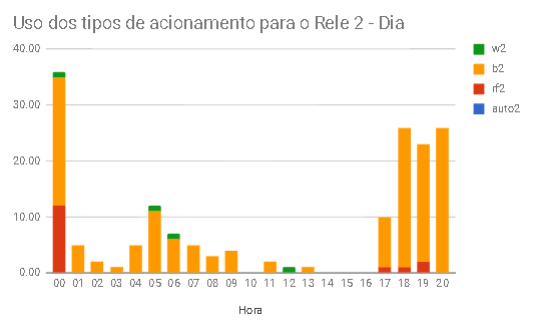
\includegraphics[width=0.8\textwidth]{usoRele2CorredorDia}
	\label{fig:usoRele2CorredorDia}
\end{figure}

\begin{figure}[H]
	\centering
	\caption{Uso do relê 2 -- Módulo do Corredor -- período}
	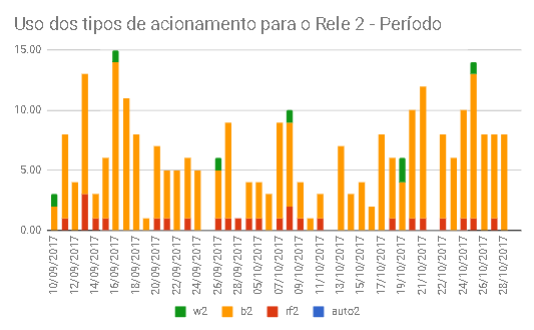
\includegraphics[width=0.8\textwidth]{UsoRele2CorredorPeriodo}
	\label{fig:UsoRele2CorredorPeriodo}
\end{figure}

\begin{figure}[H]
	\centering
	\caption{Consolidado diário -- Módulo do Corredor}
	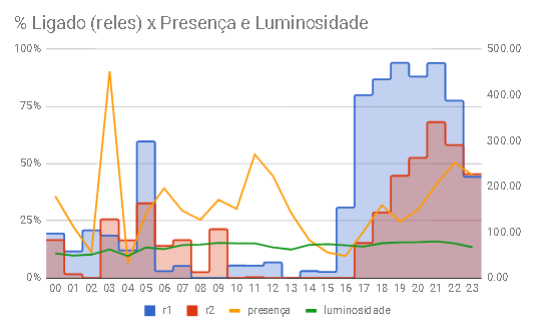
\includegraphics[width=0.8\textwidth]{RelesTempLuminosidadeCorredor}
	\label{fig:RelesTempLuminosidadeCorredor}
\end{figure}

\begin{figure}[H]
	\centering
	\caption{Resumo do Módulo da Lavanderia}
	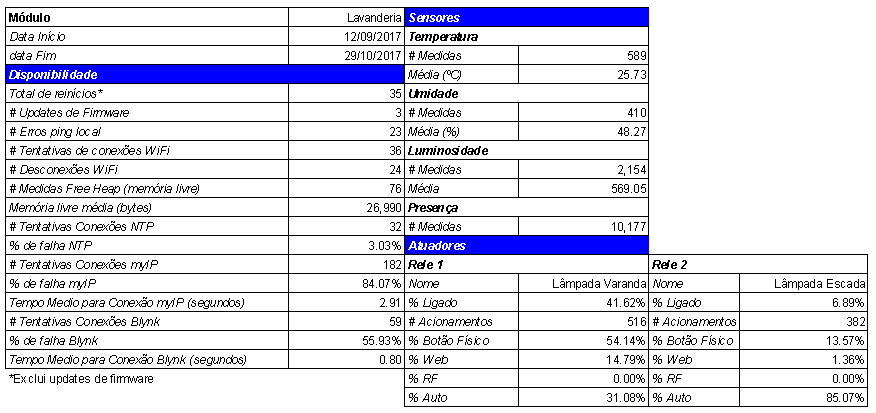
\includegraphics[width=1.0\textwidth]{resumoLavanderia}
	\label{fig:resumoLavanderia}
\end{figure}

\begin{figure}[H]
	\centering
	\caption{Disponibilidade do Módulo da Lavanderia -- dia}
	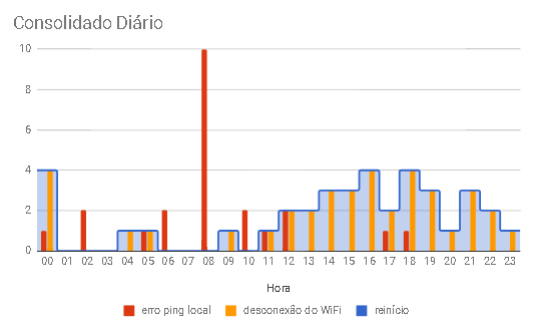
\includegraphics[width=0.8\textwidth]{lavanderiadiadisp}
	\label{fig:lavanderiadiadisp}
\end{figure}

\begin{figure}[H]
	\centering
	\caption{Disponibilidade do Módulo da Lavanderia -- período}
	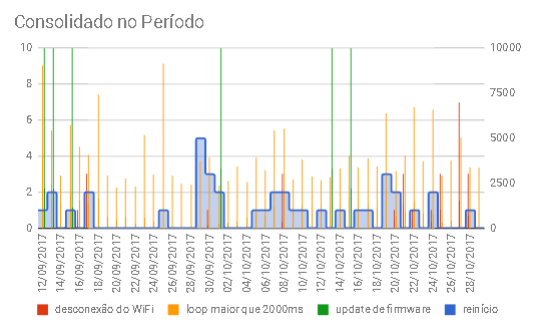
\includegraphics[width=0.8\textwidth]{lavanderiaperiododisp}
	\label{fig:lavanderiaperiododisp}
\end{figure}

\begin{figure}[H]
	\centering
	\caption{Memória livre do Módulo da Lavanderia}
	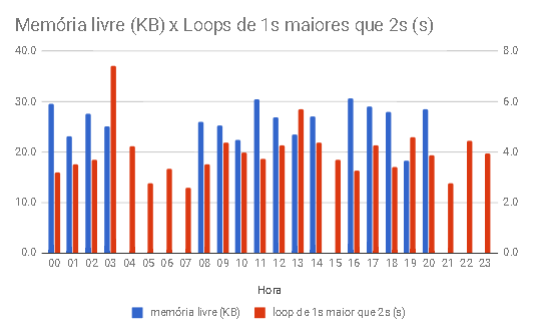
\includegraphics[width=0.8\textwidth]{memLivreLavanderia}
	\label{fig:memLivreLavanderia}
\end{figure}

\begin{figure}[H]
	\centering
	\caption{Sensores da Lavanderia -- período}
	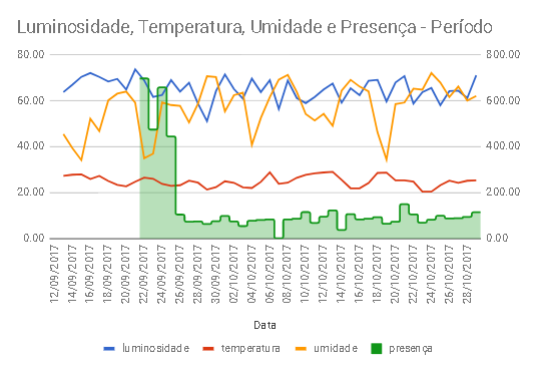
\includegraphics[width=0.8\textwidth]{lavanderiaperiodosensores}
	\label{fig:lavanderiaperiodosensores}
\end{figure}

\begin{figure}[H]
	\centering
	\caption{Sensores do Módulo da Lavanderia -- dia}
	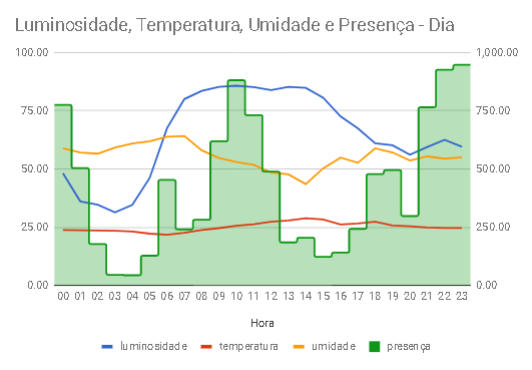
\includegraphics[width=0.8\textwidth]{lavanderiadiasensores}
	\label{fig:lavanderiadiasensores}
\end{figure}

\begin{figure}[H]
	\centering
	\caption{Uso do relê 1 do Módulo da Lavanderia -- dia}
	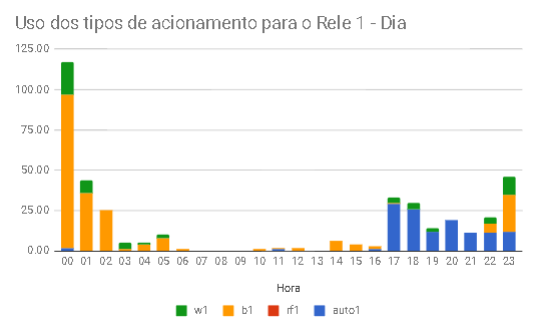
\includegraphics[width=0.8\textwidth]{usorele1Lavanderia}
	\label{fig:usorele1Lavanderia}
\end{figure}

\begin{figure}[H]
	\centering
	\caption{Uso do relê 1 do Módulo da Lavanderia -- período}
	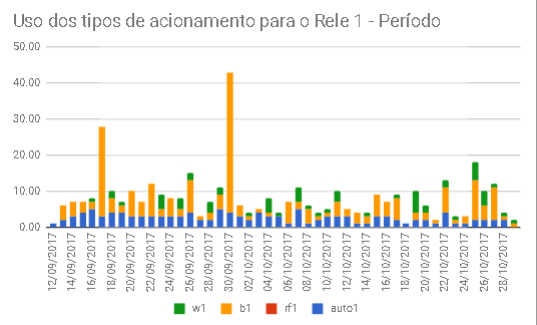
\includegraphics[width=0.8\textwidth]{Usorele1lavanderiaperiodo}
	\label{fig:Usorele1lavanderiaperiodo}
\end{figure}

\begin{figure}[H]
	\centering
	\caption{Uso do relê 2 do Módulo da Lavanderia -- dia}
	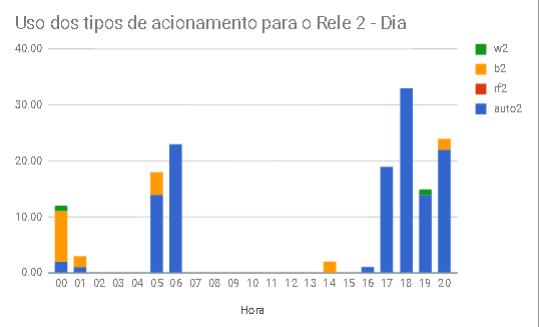
\includegraphics[width=0.8\textwidth]{UsoRele2LavanderiaDia}
	\label{fig:UsoRele2LavanderiaDia}
\end{figure}

\begin{figure}[H]
	\centering
	\caption{Uso do relê 2 do Módulo da Lavanderia -- período}
	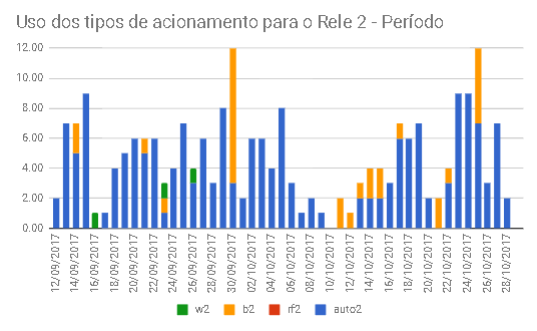
\includegraphics[width=0.8\textwidth]{UsoRele2LavanderiaPeriodo}
	\label{fig:UsoRele2LavanderiaPeriodo}
\end{figure}

\begin{figure}[H]
	\centering
	\caption{Consolidado diário do Módulo da Lavanderia}
	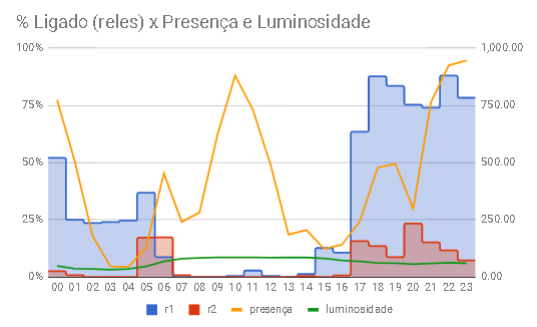
\includegraphics[width=0.8\textwidth]{RelesPresLumiLavanderia}
	\label{fig:RelesPresLumiLavanderia}
\end{figure}

\begin{figure}[H]
	\centering
	\caption{Resumo do Módulo da Sala/Cozinha}
	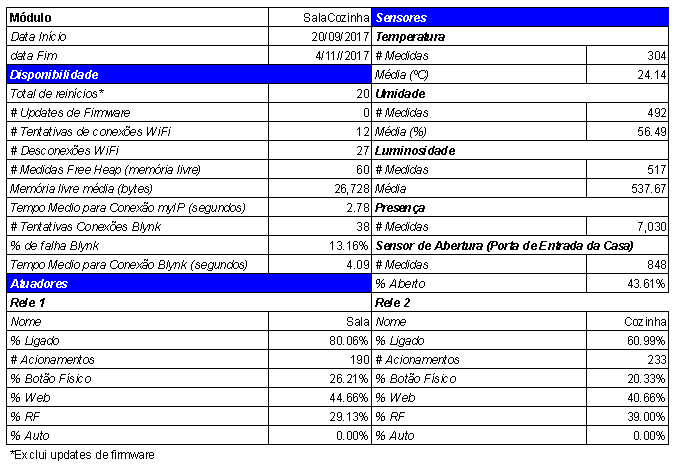
\includegraphics[width=1.0\textwidth]{resumoSalaCozinha}
	\label{fig:resumoSalaCozinha}
\end{figure}

\begin{figure}[H]
	\centering
	\caption{Disponibilidade do Módulo da Sala/Cozinha -- período}
	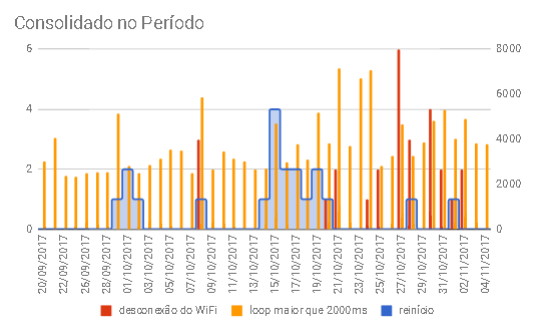
\includegraphics[width=0.8\textwidth]{salacozinhadispperiodo}
	\label{fig:salacozinhadispperiodo}
\end{figure}

\begin{figure}[H]
	\centering
	\caption{Memória livre do Módulo da Sala/Cozinha}
	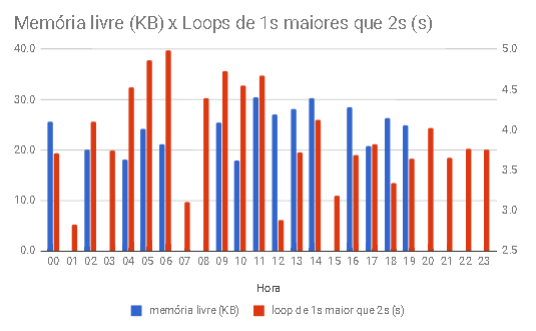
\includegraphics[width=0.8\textwidth]{memlivresalacozinha}
	\label{fig:memlivresalacozinha}
\end{figure}

\begin{figure}[H]
	\centering
	\caption{Sensores do Módulo da Sala/Cozinha -- dia}
	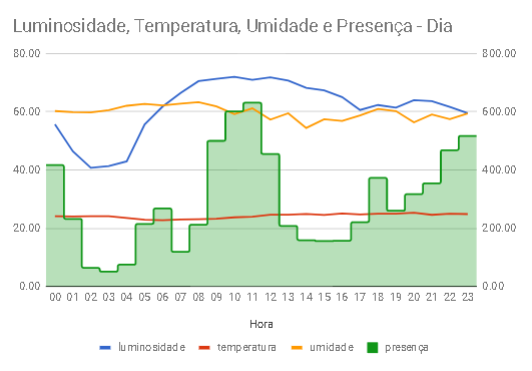
\includegraphics[width=0.8\textwidth]{sensoresdiasalacozinha}
	\label{fig:sensoresdiasalacozinha}
\end{figure}

\begin{figure}[H]
	\centering
	\caption{Sensores do Módulo da Sala/Cozinha -- período}
	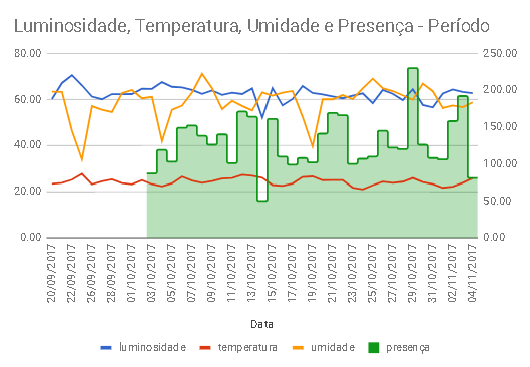
\includegraphics[width=0.8\textwidth]{sensoresperiodoSalaCozinha}
	\label{fig:sensoresperiodoSalaCozinha}
\end{figure}

\begin{figure}[H]
	\centering
	\caption{Uso do relê 1 do Módulo da Sala/Cozinha -- dia}
	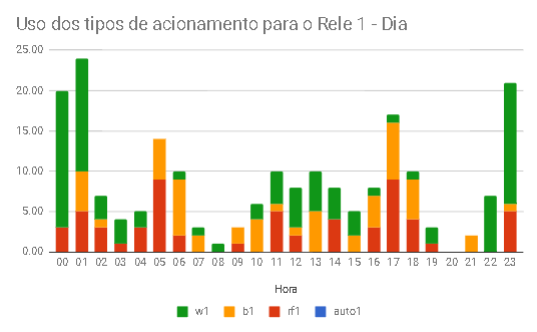
\includegraphics[width=0.8\textwidth]{usorele1salacozinhadia}
	\label{fig:usorele1salacozinhadia}
\end{figure}

\begin{figure}[H]
	\centering
	\caption{Uso do relê 1 do Módulo da Sala/Cozinha -- período}
	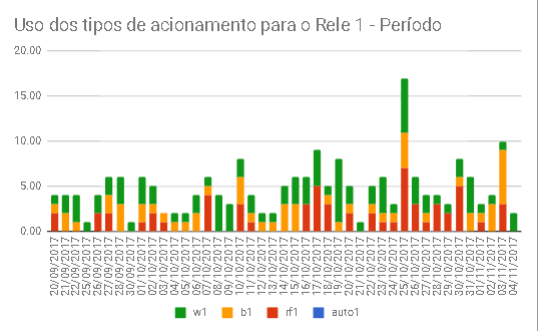
\includegraphics[width=0.8\textwidth]{usorele1salacozinhaperiodo}
	\label{fig:usorele1salacozinhaperiodo}
\end{figure}

\begin{figure}[H]
	\centering
	\caption{Uso do relê 2 do Módulo da Sala/Cozinha -- dia}
	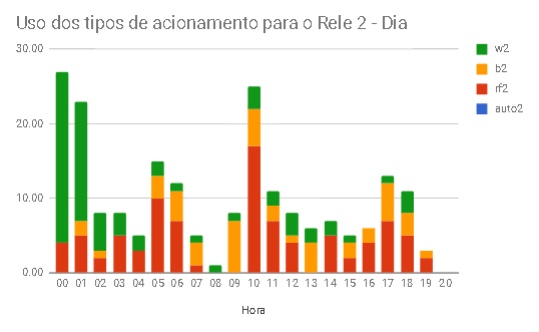
\includegraphics[width=0.8\textwidth]{usorele2salacozinhadia}
	\label{fig:usorele2salacozinhadia}
\end{figure}

\begin{figure}[H]
	\centering
	\caption{Uso do relê 2 do Módulo da Sala/Cozinha -- período}
	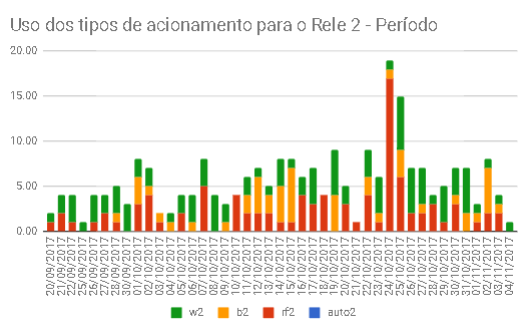
\includegraphics[width=0.8\textwidth]{usorele2salacozinhaperiodo}
	\label{fig:usorele2salacozinhaperiodo}
\end{figure}

\begin{figure}[H]
	\centering
	\caption{Porta do Módulo de Acesso -- dia}
	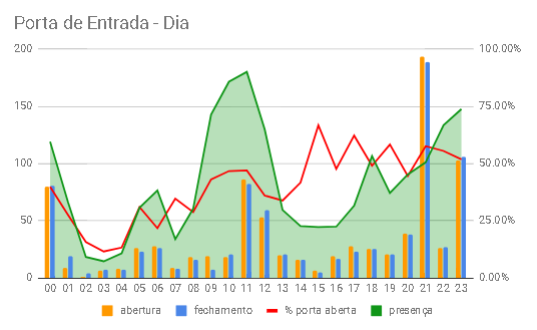
\includegraphics[width=0.8\textwidth]{portaentradadia}
	\label{fig:portaentradadia}
\end{figure}

\begin{figure}[H]
	\centering
	\caption{Porta do Módulo de Acesso -- período}
	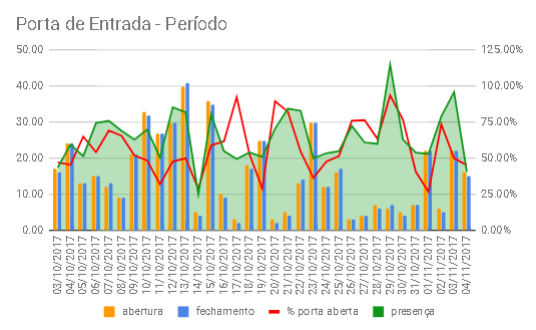
\includegraphics[width=0.8\textwidth]{portaentradaperiodo}
	\label{fig:portaentradaperiodo}
\end{figure}

\begin{figure}[H]
	\centering
	\caption{Resumo do Módulo da Entrada}
	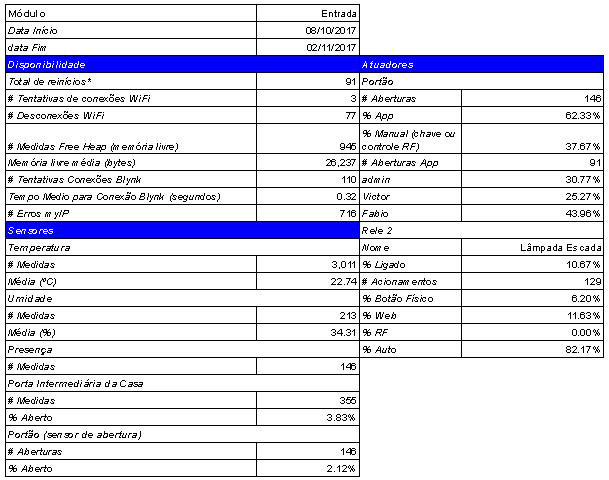
\includegraphics[width=1.0\textwidth]{resumoEntrada}
	\label{fig:resumoEntrada}
\end{figure}

\begin{figure}[H]
	\centering
	\caption{Consolidado do Módulo da Entrada -- período}
	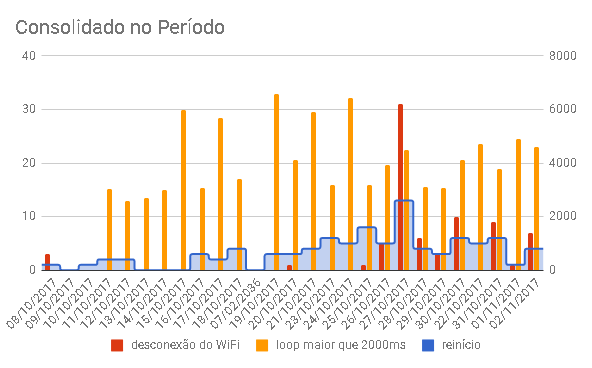
\includegraphics[width=0.8\textwidth]{entradaConsolidadoPeriodo}
	\label{fig:entradaConsolidadoPeriodo}
\end{figure}

\begin{figure}[H]
	\centering
	\caption{Memória livre do Módulo da Entrada}
	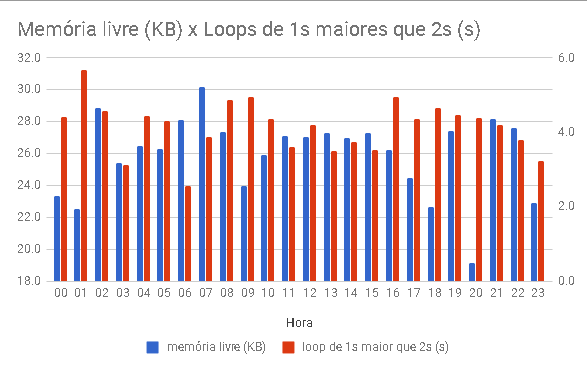
\includegraphics[width=0.8\textwidth]{memLivreEntrada}
	\label{fig:memLivreEntrada}
\end{figure}

\begin{figure}[H]
	\centering
	\caption{Sensores do Módulo da Entrada -- dia}
	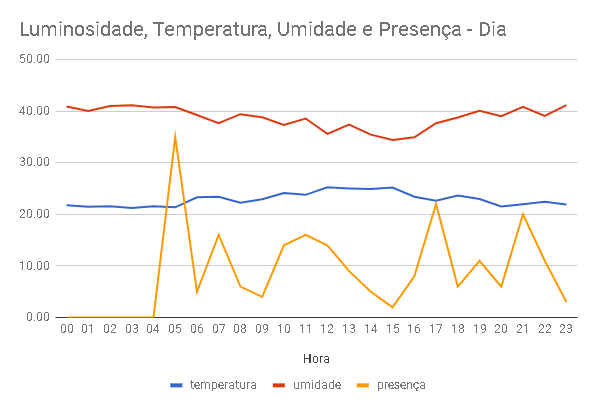
\includegraphics[width=0.8\textwidth]{sensoresEntradaDia}
	\label{fig:sensoresEntradaDia}
\end{figure}

\begin{figure}[H]
	\centering
	\caption{Sensores do Módulo da Entrada -- período}
	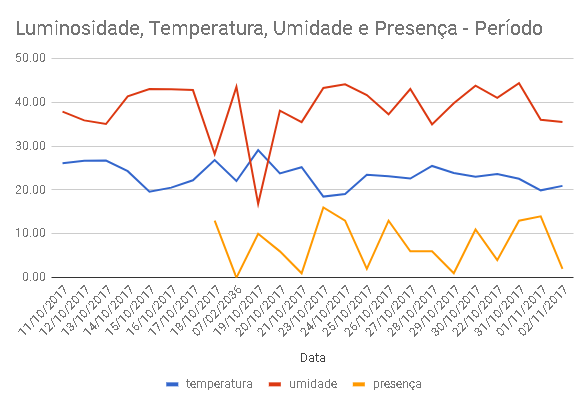
\includegraphics[width=0.8\textwidth]{sensoresEntradaPeriodo}
	\label{fig:sensoresEntradaPeriodo}
\end{figure}

\begin{figure}[H]
	\centering
	\caption{Uso da lâmpada do Módulo da Entrada -- dia}
	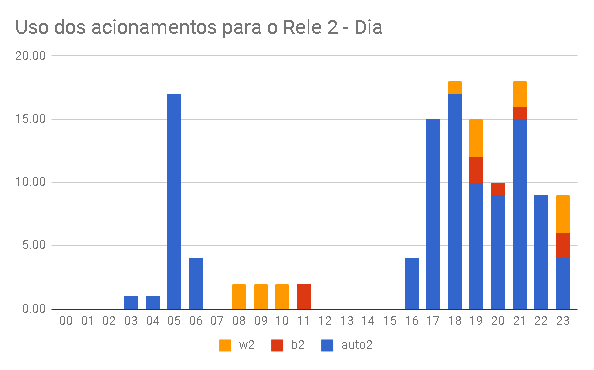
\includegraphics[width=0.8\textwidth]{usoLampadaEntradaDia}
	\label{fig:usoLampadaEntradaDia}
\end{figure}

\begin{figure}[H]
	\centering
	\caption{Uso da lâmpada do Módulo da Entrada -- período}
	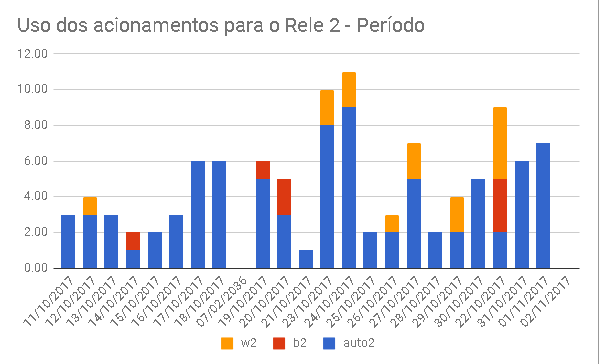
\includegraphics[width=0.8\textwidth]{UsoLampadaEntradaPeriodo}
	\label{fig:UsoLampadaEntradaPeriodo}
\end{figure}

\begin{figure}[H]
	\centering
	\caption{Uso do Módulo da Entrada -- dia}
	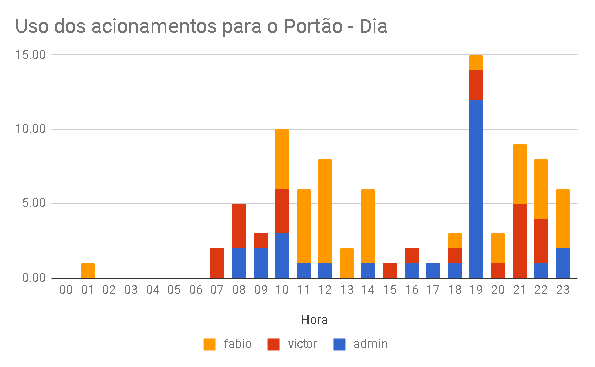
\includegraphics[width=0.8\textwidth]{usoacessodia}
	\label{fig:usoacessodia}
\end{figure}

\begin{figure}[H]
	\centering
	\caption{Uso do Módulo da Entrada -- período}
	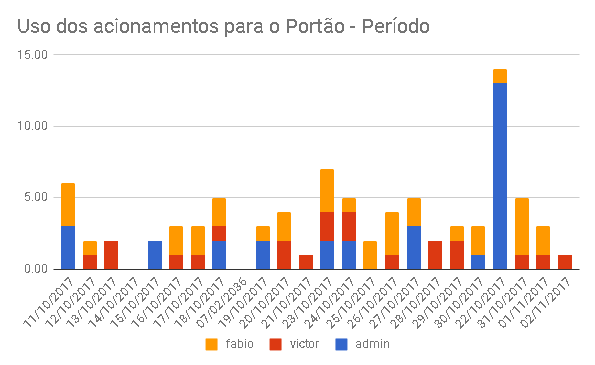
\includegraphics[width=0.8\textwidth]{usoacessoperiodo}
	\label{fig:usoacessoperiodo}
\end{figure}

\begin{figure}[H]
	\centering
	\caption{Jarinu -- consolidado por dia da semana}
	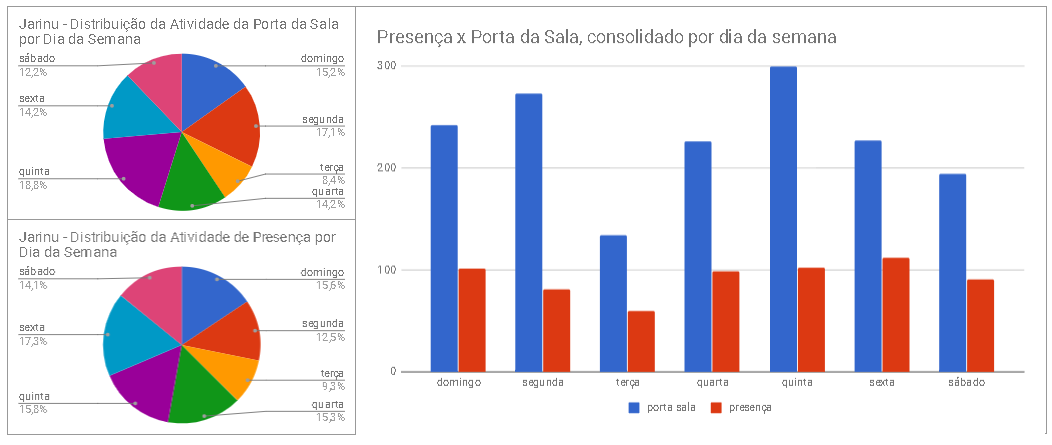
\includegraphics[width=1.0\textwidth]{JarinuDiaSemana}
	\label{fig:JarinuDiaSemana}
\end{figure}
